\chapter{Data Management Methods in blockchain}\label{chapter:data_management}

\section{Ethereum}\label{sec:}
Ethereum is considered to be a distributed transaction-based state machine  \citep{wood_2014}. There are two key components that enable Ethereum’s operation. The Ethereum Virtual Machine (EVM), which is a Turing-complete virtual machine with a simple stack-based architecture and the Ethereum blockchain, an append-only timestamped data structure where transactions and relevant information are stored. Each node that participates in the Ethereum network runs an instance of the EVM and holds a copy of the blockchain. State transitions are caused by the execution of transactions, which may result either in a transmission of value between accounts or an execution of EVM code associated with an account. Such code, known as SC, is essentially an immutable computer program that runs on top of the Ethereum protocol. Typically, SCs are written in high level programming languages, primarily in Solidity  \citep{solidity}, but must be compiled to a series of bytecode instructions in order to be executed by the EVM.

Every computation during a transaction execution is subject to a fee. This fee is predetermined  \citep{wood_2014} and paid in gas, the fundamental cost unit in Ethereum. Gas is purchased with ether prior to the transaction’s execution, at a certain gasPrice specified by the sender. Furthermore, to prevent the EVM from getting stuck in intentional or unintentional infinite loops, the notion of gasLimit was introduced. In the context of a transaction, gasLimit indicates the amount of gas the sender is willing to spend. Each block has an equivalent limit that bounds the total gas that can be used by the transactions included in it.

Since Ethereum aims to provide the necessary infrastructure for all kinds of applications, having a persistent memory area for the needs of the applications, is crucial. Indeed, every SC owns an autonomous memory area called storage, where data can be saved. Utilizing a contract’s storage also results in a gas fee. In particular, the cost of writing data on storage is proportional to the data’s size and especially high, as a means to keep the distributed database as small as possible. Consequently, storage space within the Ethereum network is a valuable resource and it should be used sparingly to store what is required for the SC's proper operation. Obviously, this limits drastically the amount of data an application can store on Ethereum. To further minimize pointless occupation of storage space, a gas refund is given when clearing an entry, i.e., setting a value from non-zero to zero.

Except for SC storage, other data structures within Ethereum’s architecture can be used as a form of cheaper data stores. In the following paragraphs we elaborate on these alternatives.

\subsection{Storing Data in SC Storage}\label{subsection:}
SC storage is a non-volatile key-value store, mapping 32-byte words to 32-byte words. Programming languages used for SC developing simplify the manipulation of storage by providing an abstraction on top of the EVM. Specifically, Solidity supports a plethora of static data types as well as some dynamic types, namely dynamic arrays and mappings.

\begin{figure}[htbp]
\centerline{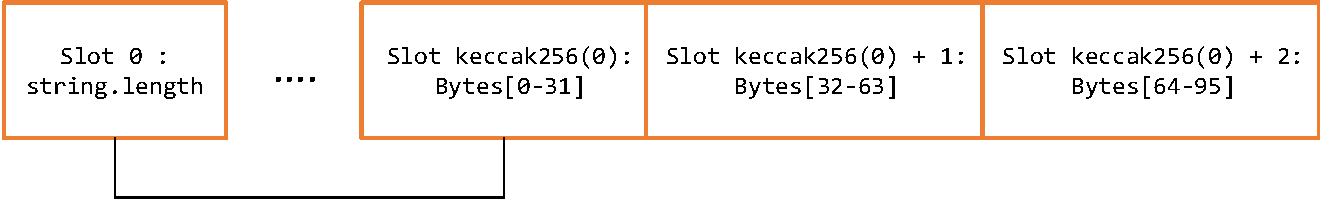
\includegraphics[width=9cm]{figs/Storage.pdf}}
\caption{Layout of dynamic arrays in SC storage.}
\label{fig:arrays}
\end{figure}

Static types are stored consecutively in storage, occupying one or more slots, depending on their size. Due to their unpredictable size, dynamic data types cannot adhere to the same principles. Regarding dynamic arrays, their starting position is determined using the keccack hash function. At first, a storage slot that holds its length is initialized at some position, p, and then the array’s data are stored starting at position keccack(p), as shown in Fig.~\ref{fig:arrays}. Solidity’s strings and bytes are special dynamic arrays with a somewhat nuanced behavior. As long as they are less than 31 bytes, their data are stored in the same position, p, as their length. When this threshold is exceeded the rules of dynamic arrays apply.

\subsection{Storing Data in Event-logs}\label{subsection:}
Every transaction receipt in the Ethereum blockchain contains log entries (logs), which are indexable checkpoints in EVM code execution  \citep{wood_2014}. In the context of Solidity, EVM’s logging operations are facilitated by the use of events. When emitting an event inside a SC, its parameters are stored in logs. Mostly, they are used as a way of triggering a change in an application’s front end or returning a value from a function  \citep{consensys}. Nonetheless, they can also be used as a means of cheaper data storage. It is noteworthy that the data stored in logs are not accessible from SCs, consequently logs cannot replace storage.

In general, logs consist of the caller’s address, a series of topics and some bytes of data. A BF is utilized to efficiently search for certain logs, based on the caller’s address and topics. When declaring an event, one can specify the keyword indexed for up to three parameters. This will result in a respective number of topics in the produced logs, allowing for a more efficient query, known as filtering. By default, both indexed and non-indexed events store the hash of their signature, which is comprised of information that can later be found in the contract’s ABI and used for filtering, as the first topic. A developer can avoid this by declaring the event as anonymous, making it less expensive to call (Table~\ref{table:event_cost}) but more difficult to retrieve.

\begin{table}[htbp]
\caption{Generalized cost model for different types of events}
\label{table:event_cost}
\resizebox{9cm}{!}{%
\begin{tabular}{@{}cccc@{}}
\toprule
 & \textbf{Indexed} & \textbf{Non-Indexed} & \textbf{Anonymous} \\ \midrule
\textbf{Topic{[}0{]}} & Signature Hash (375 gas) & Signature Hash (375 gas) & - \\
\textbf{Topic{[}1{]}} & Indexed Parameter (375 gas) & - & - \\
\textbf{Log Data} & Data (data.len*8 gas) & Data (data.len*8 gas) & Data (data.len*8 gas) \\ \bottomrule
\end{tabular}%
}
\end{table}

\subsection{Storing Data in Transaction Payload}\label{subsection:}
In Ethereum there are two types of transactions, those leading to message calls and those which result in contract creation. A message call is the act of passing some value and arbitrary binary data between accounts, either of which can be null. If the target account is a Contract Account (CA), its code is executed with the data part of the message, also termed transaction payload, as input. It is notable that transactions between Externally Owned Accounts (EOAs), may as well contain non-empty payload, transfer no value or even be self-transactions, i.e., the transaction's target is the sender.

As a rule, all transactions, including any payload, are permanently stored in the blockchain. Hence, sending data through a transaction turns out to be an alternative storage method. Considering that 16 gas is charged for every non-zero byte of a transaction’s data and 4 gas for every zero byte, this technique seems appealing. Though, one cannot ignore the fact that such data are not available inside the SC and retrieving them requires storing the corresponding transaction hash, probably in an external database as proposed by Xie et al. \citep{xie_2017}. Apart from that, a transaction payload is, at its core, a hex byte array, which implies that for more complex data types, additional logic should be implemented on the client side.

\begin{figure}[htbp]
\centerline{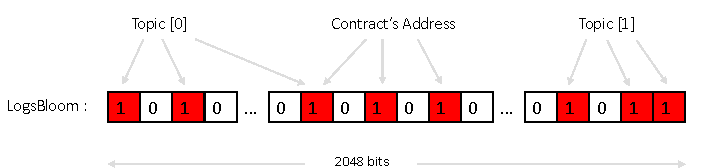
\includegraphics[width=9cm]{figs/bloom.pdf}}
\caption{Example of the bloom bits set by an event.}
\label{fig: bloom}
\end{figure}

\subsection{Storing Data in Unused Function Parameters}\label{subsection:}
With this term we refer to input data that are passed as function parameters but are no further used within function’s body, as seen in Fig.~\ref{fig:un}. This process is slightly more expensive than the previous one, as it is mandatory for function arguments to be ABI encoded, resulting in a longer payload array. However, it provides better functionality since the underlying tools for encoding and decoding such data are already developed  \citep{web3}, allowing the use of complex data types.

\begin{figure}[htbp]
\setlength{\fboxsep}{5pt}%
\setlength{\fboxrule}{0.05pt}%
\centerline{\fbox{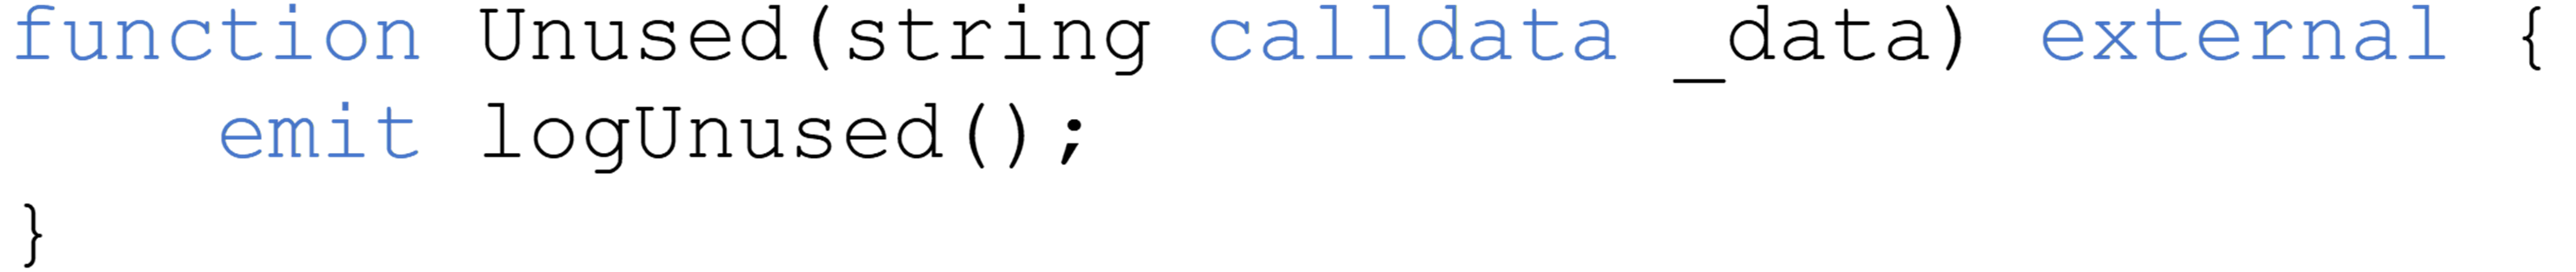
\includegraphics[width=9cm]{figs/code.png}}}
\caption{Basic example of the unused function parameters method.}
\label{fig:un}
\end{figure}

Moreover, this method includes a function call and therefore permits the execution of additional logic during the same transaction, as opposed to the aforementioned method. For instance, an event could be emitted inside the function, providing a way of future-tracking the respective transaction and retrieving its data, eliminating the need for storing the transaction hash externally.

\subsection{Retrieving logs}\label{subsection:}
In Ethereum log retrieval is accomplished with a specialized BF  \citep{wood_2014}. A BF  \citep{broder_2004} is a space-efficient probabilistic data structure used to quickly check whether an element is part of a set. 

A BF is represented by an array of m bits $\{b_1, b_2,…, b_m\}$ all initialized to zero. An element is inserted into the BF as follows. Its value is hashed k times with k independent hash functions $\{h_1, h_2,.., h_k\}$. Each time, based on the resulting hash and a mathematical formula, a bit of the BF is set to one. To determine if an element is present in the set, the same process is repeated. If all the k corresponding bits are 1s, then the element might be in the set. Otherwise, it is certainly not part of the set. In other words, a BF may return false-positives but never false negatives.

In Ethereum, every block includes a BF of 2048 bits. Each event emitted by the block’s transactions generates a log entry that sets at least three bits of the BF based on the contract’s address, and another three bits for every topic (if any), as shown in Fig.~\ref{fig: bloom}. The bits are determined by calculating the modulo 2048 of each of the first three pairs of bytes in the Keccak-256 hash of the input, where input is the contract’s address or a topic  \citep{wood_2014}.

When it comes to retrieving a specific log, each block’s BF needs to be inspected. If any of the bits that correspond to the topics or the contract’s address is zero, then, the log indeed isn’t part of the block. If all corresponding bits are set, the logs of the block are loaded and inspected individually. In case of a false positive the next block needs to be inspected.
To sum up, using BFs is much more efficient than a conventional search, but be that as it may, it is still time consuming because false positives are common and lead to additional retrievals to check if the log is the desired one. As expected, our findings (Section \ref{subsec:retrieve}) confirm that limiting the block filtering range can substantially reduce the retrieval latency.

\section{Hybrid Schemes}\label{sec:}
The Ethereum blockchain, while effective for executing code and processing data in a decentralized manner, it is not optimized for storing large volumes of data due to high costs \hl{and low space}. Consequently, in scenarios where decentralized applications must handle a lot of data, a direct on-chain storage approach isn't viable.

\begin{figure}[htbp]
\centerline{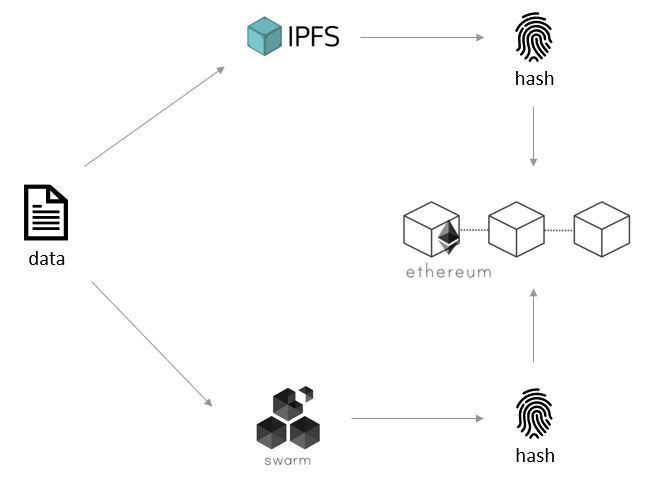
\includegraphics[width=12cm]{figs/hybrid.png}}
\caption{Hybrid architecture overview.}
\label{fig: hybrid}
\end{figure}

Distributed file systems like IPFS and Swarm can be integrated with blockchain networks like Ethereum to overcome limitations related to data storage, providing a scalable and efficient solution for fully decentralized applications. With that being said, most blockchain-based applications with high storage requirements would need to consider an on-chain/off-chain hybrid architecture.

Data storage in hybrid schemes follows a two-step approach as shown in fig. \ref{fig: hybrid}:
\begin{enumerate}
\item Data is stored in a distributed file system (IPFS or Swarm) and a unique identifier is generated for it.
\item The unique identifier is stored in the Ethereum blockchain.
\end{enumerate}

% To summarize, coupling a blockchain with a distributed file system allows for decentralized and secure storage and retrieval of data.
The immutable nature of the blockchain provides a tamper-proof way of storing the identifiers. Besides that, blockchain technology provides a built-in mechanism for timestamping (each block contains a timestamp). This can be leveraged to create provable timestamps for data stored off-chain. In conjunction with the characteristics of self-verification and authenticity that distributed file systems offer through content addressing, data integrity of such schemes is guaranteed.

When it comes to storing the identifiers in Ethereum, any of the methods that we described in the previous paragraphs can be adopted. Storing them in SC storage is the most straightforward option. On the other hand, alternatives like the event-logs, the transaction payload or the unused function arguments are far less expensive. In addition, the retrieval latency of each approach must be considered as well. Both aspects are examined and discussed in detail in the next chapter, which will hopefully enable developers to make a more informed choice.

For data retrieval, the process is simple. The DApp retrieves the identifier from the blockchain and then uses it to retrieve the actual data from the respective distributed file system.
